\chapter{用计数器设计序列发生器}

\section{什么是序列}

\textbf{序列}：一组按照预定顺序循环输出的二进制值。

例子：0110 0110 0110 ...（重复输出0, 1, 1, 0）

\begin{keypoint}[序列发生器的本质]
序列发生器 = 产生周期性重复的二进制序列的电路

$$\text{输出}(t) = \text{序列}[\text{内部状态}(t)]$$
\end{keypoint}

\section{为什么计数器可以产生序列}

计数器有一个天然能力：它按照固定的顺序经过所有状态。

序列发生器利用这一点：
\begin{enumerate}
  \item 计数器按顺序经过状态
  \item 每个状态对应序列中的一个输出值
  \item 输出逻辑 = 状态到输出的映射
\end{enumerate}

\begin{center}
\begin{tikzpicture}
  \node[draw, minimum width=2.5cm, minimum height=1.2cm] (cnt) at (0,0) {计数器};
  \node[draw, minimum width=2.5cm, minimum height=1.2cm] (map) at (4,0) {输出映射};

  \draw[->] (cnt) -- (map) node[midway,above] {状态};
  \draw[->] (map) -- ++(1.5,0) node[right] {序列输出};

  \node at (2,-1.5) {计数器提供"顺序"，映射提供"每个状态的输出值"};
\end{tikzpicture}
\end{center}

\section{方案1：计数器 + 组合逻辑映射}

\subsection{设计序列：0110 0110 0110 ...}

序列长度L=4，重复：0, 1, 1, 0。

\begin{enumerate}
  \item 使用模4计数器（状态：0, 1, 2, 3, 0, 1, ...）
  \item 输出映射表：
\end{enumerate}

\begin{center}
\begin{tabular}{|c|c|}
\hline
\textbf{计数器状态} & \textbf{输出} \\
\hline
0(00) & 0 \\
1(01) & 1 \\
2(10) & 1 \\
3(11) & 0 \\
\hline
\end{tabular}
\end{center}

逻辑表达式：$output = \overline{Q_1} \cdot Q_0 + Q_1 \cdot \overline{Q_0}$（即 $Q_1 \oplus Q_0$）

\begin{lstlisting}[caption={序列0110发生器（计数器+组合逻辑）}]
library ieee;
use ieee.std_logic_1164.all;
use ieee.std_logic_unsigned.all;

entity seq_gen_0110 is
  port (
    clk   : in  std_logic;
    rst_n : in  std_logic;
    seq_out : out std_logic
  );
end seq_gen_0110;

architecture rtl of seq_gen_0110 is
  signal cnt : std_logic_vector(1 downto 0);  -- 模4计数器
begin
  -- 模4计数器
  process(clk, rst_n)
  begin
    if rst_n = '0' then
      cnt <= (others => '0');
    elsif rising_edge(clk) then
      if cnt = "11" then
        cnt <= (others => '0');
      else
        cnt <= cnt + 1;
      end if;
    end if;
  end process;

  -- 输出映射：状态0和3输出0，状态1和2输出1
  -- 即：Q1 XOR Q0
  seq_out <= cnt(1) xor cnt(0);
end rtl;
\end{lstlisting}

\section{方案2：状态机型序列发生器}

同样的序列可以用状态机实现：

\begin{center}
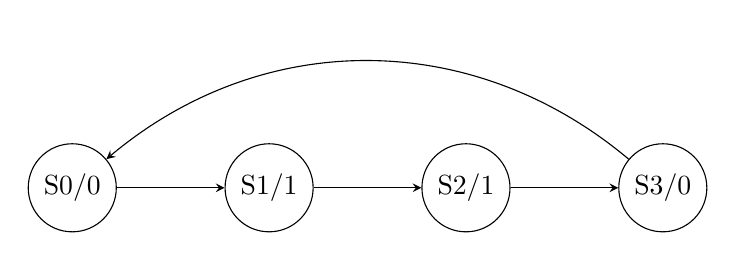
\begin{tikzpicture}[->, >=stealth, node distance=2.5cm, auto]
  \node[draw, circle] (S0) at (0,0) {S0/0};
  \node[draw, circle] (S1) at (2.5,0) {S1/1};
  \node[draw, circle] (S2) at (5,0) {S2/1};
  \node[draw, circle] (S3) at (7.5,0) {S3/0};

  \draw (S0) -- (S1);
  \draw (S1) -- (S2);
  \draw (S2) -- (S3);
  \draw (S3) edge[bend right=40] (S0);
\end{tikzpicture}
\end{center}

\begin{lstlisting}[caption={序列0110发生器（状态机版本）}]
architecture fsm of seq_gen_0110 is
  type state_type is (S0, S1, S2, S3);
  signal state : state_type;
begin
  process(clk, rst_n)
  begin
    if rst_n = '0' then
      state <= S0;
    elsif rising_edge(clk) then
      case state is
        when S0 => state <= S1;
        when S1 => state <= S2;
        when S2 => state <= S3;
        when S3 => state <= S0;
      end case;
    end if;
  end process;

  -- 输出逻辑
  seq_out <= '0' when (state = S0 or state = S3) else '1';
end fsm;
\end{lstlisting}

\section{方案3：移位寄存器型序列发生器}

有些序列恰好可以用移位寄存器+反馈产生。例如伪随机序列（LFSR）。

这将在第六部分（移位寄存器）和第七部分（环形计数器）中详细展开。

\section{方案4：ROM/查找表型序列发生器}

适用于长序列：
\begin{itemize}
  \item 将整个序列预存在ROM中
  \item 计数器作为ROM的地址
  \item ROM输出 = 序列值
\end{itemize}

\section{方案比较}

\begin{center}
\begin{tabular}{|l|c|c|c|}
\hline
\textbf{方案} & \textbf{适用场景} & \textbf{优点} & \textbf{缺点} \\
\hline
计数器+MUX & 序列有规律 & 资源少 & 需要推导逻辑 \\
状态机 & 任意序列 & 通用 & 状态多时复杂 \\
移位寄存器 & LFSR/循环型 & 结构规整 & 仅限特定类型 \\
ROM/查找表 & 长序列 & 通用 & 资源多（需要ROM） \\
\hline
\end{tabular}
\end{center}

\section{考试常见变式}

\begin{enumerate}
  \item \textbf{变式1：设计任意周期性的序列}

  例：产生序列 10110 10110 ...（长度5）
  解：模5计数器 + 状态到输出映射表

  \item \textbf{变式2：多路输出序列}

  同时输出多个相关序列（如正交序列）

  \item \textbf{变式3：伪随机序列（LFSR）}

  用移位寄存器+反馈产生看似随机的序列。这是通信系统中的重要应用。

  \item \textbf{变式4：可配置的序列发生器}

  序列可以动态改变（通过改变映射表或ROM内容）
\end{enumerate}

\begin{examtip}[序列发生器秒杀法]
1. 确定序列长度L
2. 设计模L计数器
3. 建立状态→输出映射表（真值表）
4. 推导输出逻辑（或用case直接写）

\textbf{计数器+case语句是最通用的解法，适用于任何序列。}
\end{examtip}

\section{变式详解}
\chapter{序列发生器——全部变式详解}

\section{变式1：任意周期序列（计数器+映射表）}

\begin{detailbox}[完整教学]
\textbf{【通用方案】}模L计数器+状态→输出映射表。
\textbf{【例题】}产生序列10110(长度5)。模5计数器+case映射：
\begin{lstlisting}
case cnt is
  when "000" => seq <= '1';
  when "001" => seq <= '0';
  when "010" => seq <= '1';
  when "011" => seq <= '1';
  when "100" => seq <= '0';
end case;
\end{lstlisting}
\textbf{【适用范围】}任意序列。长度L→模L计数器。
\end{detailbox}


\section{变式2：状态机型序列发生器}

\begin{detailbox}[完整教学]
\textbf{【方案】}每个状态输出一个序列值。状态转移=序列顺序。
\textbf{【优点】}状态名有意义（如"S\_1","S\_0","S\_1","S\_1","S\_0"）。但状态多时代码冗长。
\textbf{【比较】}推荐用计数器+case——代码更简洁。
\end{detailbox}


\section{变式3：移位寄存器+LFSR发生器}

\begin{detailbox}[完整教学]
\textbf{【LFSR】}线性反馈移位寄存器。反馈=选择位的XOR。
\textbf{【应用】}伪随机序列(PRBS)、CRC、扰码。
\textbf{【4位LFSR(X4+X3+1)】}反馈=Q3 xor Q2。产生15个伪随机状态。
\textbf{【注意】}全0状态非法——LFSR会锁死在0000。必须初始化为非0值。
\end{detailbox}


\section{变式4：ROM/查找表型序列发生器}

\begin{detailbox}[完整教学]
\textbf{【方案】}预存整个序列在ROM中。计数器=地址。
\textbf{【优点】}任意序列、可重配置。适合长序列。
\textbf{【VHDL】}
\begin{lstlisting}
type rom_type is array (0 to 15) of std_logic_vector(3 downto 0);
constant SEQ_ROM : rom_type := (x"1", x"0", x"1", x"1", x"0", ...);
seq <= SEQ_ROM(to_integer(unsigned(cnt)));
\end{lstlisting}
\end{detailbox}
